% Options for packages loaded elsewhere
\PassOptionsToPackage{unicode}{hyperref}
\PassOptionsToPackage{hyphens}{url}
\PassOptionsToPackage{dvipsnames,svgnames,x11names}{xcolor}
\documentclass[
  11pt,
]{article}
\usepackage{xcolor}
\usepackage[margin=1in]{geometry}
\usepackage{amsmath,amssymb}
\setcounter{secnumdepth}{-\maxdimen} % remove section numbering
\usepackage{iftex}
\ifPDFTeX
  \usepackage[T1]{fontenc}
  \usepackage[utf8]{inputenc}
  \usepackage{textcomp} % provide euro and other symbols
\else % if luatex or xetex
  \usepackage{unicode-math} % this also loads fontspec
  \defaultfontfeatures{Scale=MatchLowercase}
  \defaultfontfeatures[\rmfamily]{Ligatures=TeX,Scale=1}
\fi
\usepackage{lmodern}
\ifPDFTeX\else
  % xetex/luatex font selection
\fi
% Use upquote if available, for straight quotes in verbatim environments
\IfFileExists{upquote.sty}{\usepackage{upquote}}{}
\IfFileExists{microtype.sty}{% use microtype if available
  \usepackage[]{microtype}
  \UseMicrotypeSet[protrusion]{basicmath} % disable protrusion for tt fonts
}{}
\makeatletter
\@ifundefined{KOMAClassName}{% if non-KOMA class
  \IfFileExists{parskip.sty}{%
    \usepackage{parskip}
  }{% else
    \setlength{\parindent}{0pt}
    \setlength{\parskip}{6pt plus 2pt minus 1pt}}
}{% if KOMA class
  \KOMAoptions{parskip=half}}
\makeatother
\usepackage{longtable,booktabs,array}
\newcounter{none} % for unnumbered tables
\usepackage{calc} % for calculating minipage widths
% Correct order of tables after \paragraph or \subparagraph
\usepackage{etoolbox}
\makeatletter
\patchcmd\longtable{\par}{\if@noskipsec\mbox{}\fi\par}{}{}
\makeatother
% Allow footnotes in longtable head/foot
\IfFileExists{footnotehyper.sty}{\usepackage{footnotehyper}}{\usepackage{footnote}}
\makesavenoteenv{longtable}
\usepackage{graphicx}
\makeatletter
\newsavebox\pandoc@box
\newcommand*\pandocbounded[1]{% scales image to fit in text height/width
  \sbox\pandoc@box{#1}%
  \Gscale@div\@tempa{\textheight}{\dimexpr\ht\pandoc@box+\dp\pandoc@box\relax}%
  \Gscale@div\@tempb{\linewidth}{\wd\pandoc@box}%
  \ifdim\@tempb\p@<\@tempa\p@\let\@tempa\@tempb\fi% select the smaller of both
  \ifdim\@tempa\p@<\p@\scalebox{\@tempa}{\usebox\pandoc@box}%
  \else\usebox{\pandoc@box}%
  \fi%
}
% Set default figure placement to htbp
\def\fps@figure{htbp}
\makeatother
\setlength{\emergencystretch}{3em} % prevent overfull lines
\providecommand{\tightlist}{%
  \setlength{\itemsep}{0pt}\setlength{\parskip}{0pt}}
\usepackage{amssymb}
\usepackage{newunicodechar}
\newunicodechar{²}{\textsuperscript{2}}
\newunicodechar{≈}{\ensuremath{\approx}}
\newunicodechar{≤}{\ensuremath{\le}}
\newunicodechar{≥}{\ensuremath{\ge}}
\newunicodechar{−}{\ensuremath{-}}
\newunicodechar{×}{\ensuremath{\times}}
\newunicodechar{→}{\ensuremath{\to}}
\newunicodechar{α}{\ensuremath{\alpha}}
\newunicodechar{Δ}{\ensuremath{\Delta}}
\newunicodechar{ℝ}{\ensuremath{\mathbb{R}}}
\newunicodechar{∈}{\ensuremath{\in}}
\newunicodechar{ᵀ}{\ensuremath{^{\top}}}
\newunicodechar{′}{\ensuremath{'}}
\newunicodechar{⁻}{\ensuremath{^{-}}}
\newunicodechar{¹}{\textsuperscript{1}}
\newunicodechar{³}{\textsuperscript{3}}
\newunicodechar{½}{\ensuremath{\tfrac12}}
\newunicodechar{¼}{\ensuremath{\tfrac14}}
\newunicodechar{¾}{\ensuremath{\tfrac34}}
\newunicodechar{°}{\ensuremath{^\circ}}
\newunicodechar{⁰}{\textsuperscript{0}}
\newunicodechar{₂}{\ensuremath{_2}}
\newunicodechar{·}{\ensuremath{\cdot}}
\newunicodechar{✓}{\checkmark}
\usepackage{bookmark}
\IfFileExists{xurl.sty}{\usepackage{xurl}}{} % add URL line breaks if available
\urlstyle{same}
\hypersetup{
  pdftitle={The Model Knows Better Than It Answers: Gemma 3 Composes a Spatial Map Its Answers Never Read},
  pdfauthor={Cristhian Gómez Neira},
  colorlinks=true,
  linkcolor={Maroon},
  filecolor={Maroon},
  citecolor={Blue},
  urlcolor={Blue},
  pdfcreator={LaTeX via pandoc}}

\title{The Model Knows Better Than It Answers: Gemma 3 Composes a
Spatial Map Its Answers Never Read}
\author{Cristhian Gómez Neira}
\date{}

\begin{document}
\maketitle
\begin{abstract}
When people read ``A is 3 units north of B; C is 2 units east of A'',
they can answer questions the text never answers, as if looking at a
picture. We ask whether a language model builds such a picture, and
whether its answers use it. On text-only layouts, Gemma 3 12B builds a
map: linear probes read each object's position from its activations (R²
= 0.74), including positions that require combining sentences. But the
answers do not use this map. Erasing it everywhere costs no more
accuracy than erasing random directions. Instead, the answers depend on
a small 2-D code over the sentence that states each position. Swapping
it moves 72\% of the affected answers (83\% in Gemma 3 27B; random:
0\%), and it acts as a switch, not a coordinate. The answers also use
the chain of relations only partly, so answering from the model's own
unused map beats the model on chain questions (0.80 vs 0.73). The main
tests were preregistered.
\end{abstract}

\section{1. Introduction}\label{introduction}

Does a language model solve a spatial puzzle by consulting something
like a map, or by chaining the relations it was told? Written reasoning
cannot settle this, because it contains only words. The question is
about the format of the model's internal computation.

Geometry can be read out of language models. Probes recover the
coordinates of real places (Gurnee \& Tegmark, 2023), circular codes for
days and months (Engels et al., 2024), and spatial relations in
described scenes (Tehenan et al., 2025). Whether such representations
are used is less clear. An et al.~(2026) find spatial information that
``can causally influence behavior'' but is ``weakly integrated into
final predictions''. Probing alone cannot answer the question: a probe
shows that information is present, not that the model relies on it
(Hewitt \& Liang, 2019).

We test use directly. If a model answers from a map, then editing one
object's position in that map should move every spatial answer
consistently, and removing the map should hurt. We find the opposite.
The map is real and accurate, but the answers come from a different
route. Our contributions:

\begin{itemize}
\tightlist
\item
  A text-only layout task, with a behaviour test that selects a model
  able to solve it without written reasoning.
\item
  Evidence that Gemma 3 12B composes object positions across sentences,
  including distances that rule out simple copying of the stated
  offsets.
\item
  Evidence that the answers do not use this map: copying it, steering it
  and erasing it all leave the answers unchanged, also on harder
  4--5-object scenes.
\item
  A small 2-D code at each stated sentence that does control the
  answers, confirmed on fresh data and replicated in Gemma 3 27B. It
  behaves like a switch, not a coordinate.
\item
  A mechanism: the question reads each object's own sentence, never the
  map, and uses the chain only partly. Answering from the unused map
  would be more accurate on chain questions, but pointing the model's
  attention at the map does not help.
\end{itemize}

\section{2. Setup}\label{setup}

\textbf{Scenes and questions.} Each scene places three named objects on
an integer grid, using relations such as ``Cy is 2 units east of Ana''.
One object is the root. An object placed relative to an object that is
itself placed relative to the root is two steps away; its position
follows only by combining two sentences. After the description, the
prompt lists the objects (``The objects are: Ana, Bo, Cy.''). Questions
ask which object is farthest from or closest to another, the compass
direction from one object to another, and which of two objects is
further north or further east. We score each allowed answer by its
log-probability, without generation. Correct answers win by at least 1
unit (10° for direction).

\textbf{Model.} We screened eight open models (Qwen3 1.7B--14B, Llama
3.2 3B, Gemma 3 4B--27B) with a preregistered behaviour test. The
smallest model that solved 3-object scenes reliably without written
reasoning was \textbf{Gemma 3 12B} (accuracy 0.76 {[}0.74, 0.77{]}; Fig.
1). Gemma 3 27B served as a replication. One question type (``Is Y
closer to X than Z?'') was at chance for every model and was excluded.

\begin{figure}
\centering
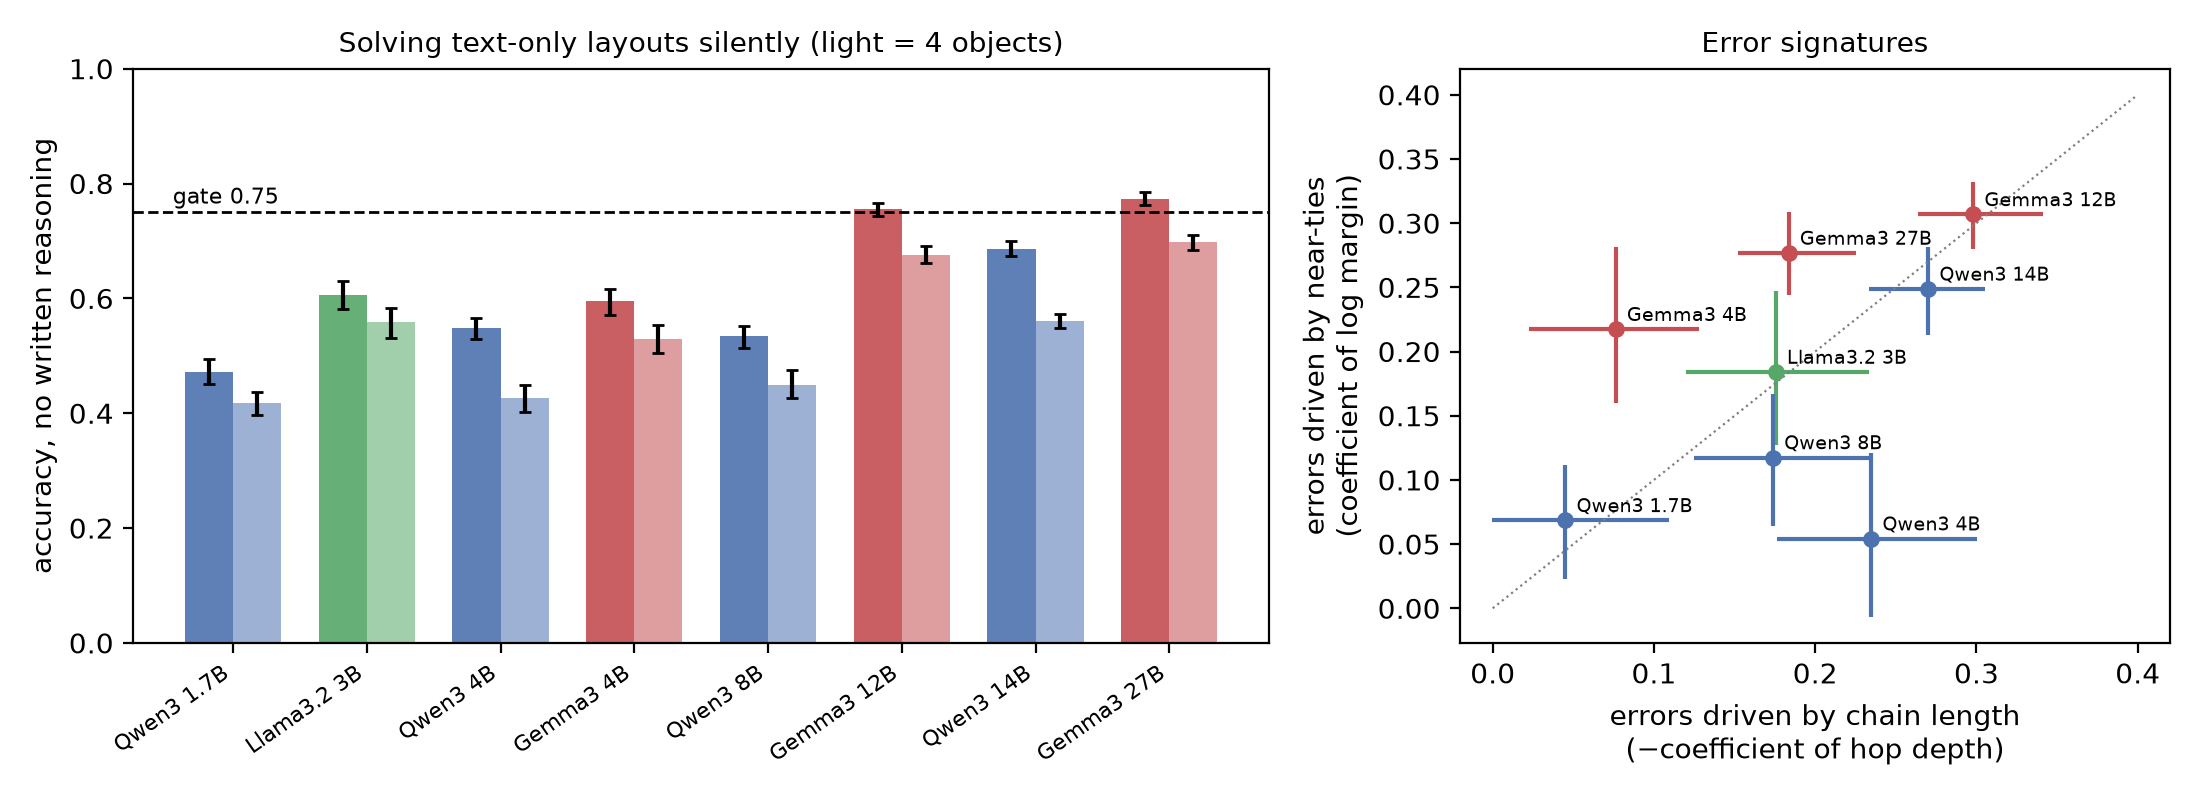
\includegraphics[width=1\linewidth,height=\textheight,keepaspectratio,alt={Left: accuracy without written reasoning (dashed line: the preregistered threshold). Qwen models put little probability on one-word answers, so their accuracies are lower bounds. Right: errors grow with chain depth and with how close the competing answers are.}]{figures/fig1_behaviour.png}
\caption{Left: accuracy without written reasoning (dashed line: the
preregistered threshold). Qwen models put little probability on one-word
answers, so their accuracies are lower bounds. Right: errors grow with
chain depth and with how close the competing answers are.}
\end{figure}

\textbf{Methods.} We use four kinds of tools.

\begin{itemize}
\tightlist
\item
  \emph{Probes:} ridge regressions that read each object's (x, y) from
  the residual stream at its name in the object list, with
  shuffled-label, layer-0 and random-model controls.
\item
  \emph{Activation patching:} run the model on one scene but copy in
  hidden states from a scene where one object sits elsewhere.
\item
  \emph{Distributed alignment search} (DAS; Geiger et al., 2024): learn
  a 2-D subspace whose swap moves the answers.
\item
  \emph{Erasure:} iterative nullspace projection (Ravfogel et al., 2020)
  removes the directions a probe reads.
\end{itemize}

Unless stated otherwise, causal metrics compare the edited answer with
the answer the model itself gives on the scene being imitated.

\textbf{Preregistration.} We committed hypotheses, metrics and decision
rules to version control before collecting each dataset. Section 6 lists
every test, its verdict, and which analyses were exploratory.

\section{3. Results}\label{results}

\subsection{3.1 The model builds a map}\label{the-model-builds-a-map}

A linear probe at the object list reads each object's position. Accuracy
is near zero up to layer 11, rises sharply at layers 12--13, and peaks
at \textbf{layer 21 (R² = 0.74 {[}0.72, 0.75{]})}. All controls score
0.00 (Fig. 2a).

Objects two steps from the root are read as well as one-step objects
(0.74 vs 0.76). A baseline that knows only each object's own stated
offset reaches 0.22 on them, so the model combines the sentences. It
also computes something beyond a sum of offsets. A probe for distance to
the root reaches \textbf{R² = 0.62 {[}0.56, 0.67{]}} on two-step
objects, while the best additive baseline built from both stated offsets
scores −0.05. The same coordinates can be read at the object's name
inside a question and at the end of its own sentence.

\subsection{3.2 The answers do not use the
map}\label{the-answers-do-not-use-the-map}

We tried to make the answers follow the map in four ways. None worked.

\begin{itemize}
\tightlist
\item
  \textbf{Copying.} Copying an object's list representation from a scene
  where it sits elsewhere changes no answer: 0.00 {[}0.00, 0.00{]} on
  390 pairs. Copying its name inside the question also gives 0.00.
\item
  \textbf{Steering.} Moving the list representation along the probe's
  (x, y) directions, over ±5 units, flips an answer in only 2\% of the
  268 sweeps where geometry says an answer must flip.
\item
  \textbf{A learned 2-D subspace at the list.} DAS at the object list
  reaches only 0.07 {[}0.05, 0.09{]}.
\item
  \textbf{Erasure.} We removed the probe-readable coordinates at every
  token, at layer 14, 21 or 28 alone, or at all layers 12--30. After
  erasure the probe's R² is at most 0.09 (down from up to 0.69). On 300
  new scenes, erasing the map hurts questions about two-step objects no
  more than erasing random directions of the same rank. The excess drop
  ranges from −0.027 to −0.003, and no confidence interval rises above
  0.001 (Fig. 3).
\end{itemize}

The last test could fail simply because three-object scenes are easy to
answer by chaining. We therefore repeated the erasure on 4--5-object
scenes, where questions can need up to four chained relations. The model
still had room to fail: it answered deep questions with accuracy 0.65,
against about 0.36 for chance. Erasing the map again did not hurt deep
questions more than random erasure. The largest effect, 0.023 {[}0.004,
0.041{]} at layer 21, is a fifth of the preregistered threshold of 0.10.

Where does the information go instead? Copying an object's whole
\emph{sentence} moves almost all answers at layer 6 (0.94). This effect
fades between layers 16 and 32, and over the same layers the question
tokens take it over (0.78 by layer 32; Fig. 2b). The information flows
from the stated sentences into the question and bypasses the object
list.

\begin{figure}
\centering
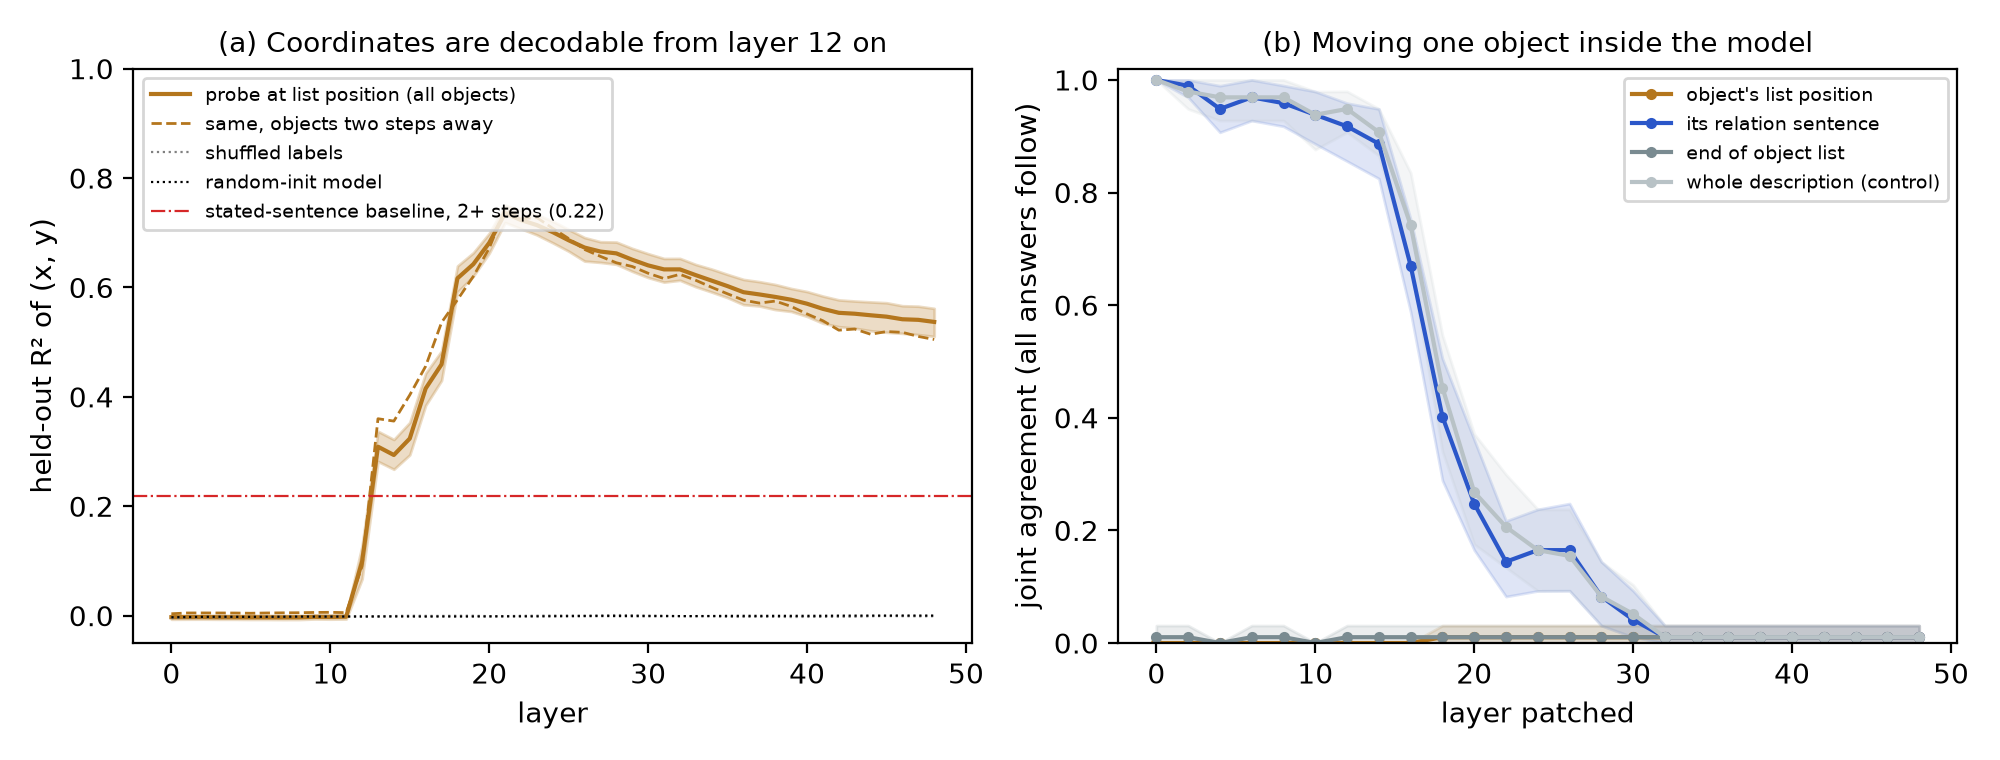
\includegraphics[width=1\linewidth,height=\textheight,keepaspectratio,alt={(a) Probe R² for (x, y) at the object list, by layer, with controls and the stated-sentence baseline. (b) Share of pairs in which every answer follows the copied site, by site and layer (100 pairs).}]{figures/fig2_mechanism.png}
\caption{(a) Probe R² for (x, y) at the object list, by layer, with
controls and the stated-sentence baseline. (b) Share of pairs in which
every answer follows the copied site, by site and layer (100 pairs).}
\end{figure}

\begin{figure}
\centering
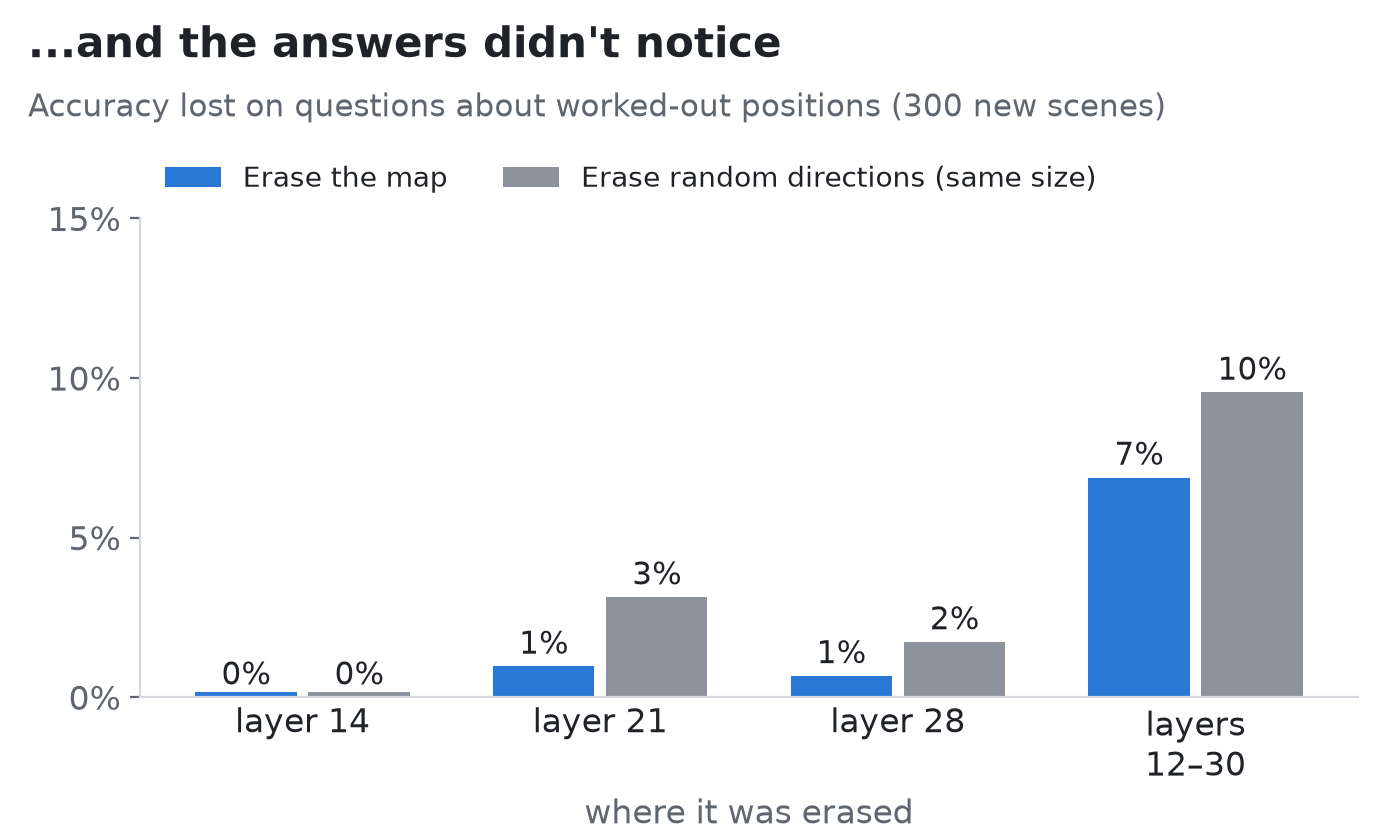
\includegraphics[width=1\linewidth,height=\textheight,keepaspectratio,alt={Accuracy lost on questions about two-step objects when the map is erased, compared with erasing random directions of the same size (Gemma 3 12B, 300 new scenes).}]{figures/fig3_erasure.png}
\caption{Accuracy lost on questions about two-step objects when the map
is erased, compared with erasing random directions of the same size
(Gemma 3 12B, 300 new scenes).}
\end{figure}

\subsection{3.3 What the answers use instead: a 2-D switch at each
sentence}\label{what-the-answers-use-instead-a-2-d-switch-at-each-sentence}

Since the sentence carries the information, we searched for a compact
code there. In an exploratory run, a 2-D subspace at layer 14 of the
moved object's sentence moved 0.81 of the affected answers. We then
fixed the site, layer and decision rule in advance and reran on fresh
scenes, adding Gemma 3 27B at the matching relative depth.

{\def\LTcaptype{none} % do not increment counter
\begin{longtable}[]{@{}
  >{\raggedright\arraybackslash}p{(\linewidth - 4\tabcolsep) * \real{0.3333}}
  >{\raggedright\arraybackslash}p{(\linewidth - 4\tabcolsep) * \real{0.3333}}
  >{\raggedright\arraybackslash}p{(\linewidth - 4\tabcolsep) * \real{0.3333}}@{}}
\toprule\noalign{}
\begin{minipage}[b]{\linewidth}\raggedright
\end{minipage} & \begin{minipage}[b]{\linewidth}\raggedright
Gemma 3 12B (layer 14)
\end{minipage} & \begin{minipage}[b]{\linewidth}\raggedright
Gemma 3 27B (layer 18)
\end{minipage} \\
\midrule\noalign{}
\endhead
\bottomrule\noalign{}
\endlastfoot
Learned 2-D code, all questions & \textbf{0.72 {[}0.68, 0.75{]}} &
\textbf{0.83 {[}0.80, 0.85{]}} \\
Random 2-D code & 0.00 & 0.00 \\
Further north / further east & 0.94 / 0.90 & 0.94 / 0.84 \\
Direction & 0.60 & 0.81 \\
Closest / farthest & 0.38 / 0.33 & 0.43 / 0.38 \\
\end{longtable}
}

Both runs pass the preregistered rule. The code works best for
one-coordinate questions, and worst for closest and farthest, which
depend on every object at once. Three checks suggest it is a genuine
part of the computation rather than an artefact of the method (Makelov
et al., 2024).

\begin{itemize}
\tightlist
\item
  \emph{Stability.} Two independent trainings on disjoint data find
  overlapping planes (principal angles 47° and 56°; random planes never
  exceed a cosine of 0.07).
\item
  \emph{Competence.} The edit succeeds more often where the model itself
  answers correctly (0.75 vs 0.48 in 12B).
\item
  \emph{Write-in.} Setting the code from the stated offset, instead of
  copying it from another run, still moves 0.27 of the answers, against
  0.00 for a random subspace.
\end{itemize}

\textbf{It is a switch, not a dial.} If the two numbers were
coordinates, setting them halfway between two layouts should move the
object halfway. We tested this on questions whose answer at the halfway
position differs from both stated layouts. The model rarely gives that
in-between answer: \textbf{0.085 in 12B and 0.055 in 27B, below the
0.141 expected by chance}. Instead it snaps to one of the two stated
layouts (Fig. 4b). Consistent with this, the code does not change
linearly with the stated distance: a linear fit explains it no better
than for random directions (R² 0.31 vs a 95th percentile of 0.35).

\begin{figure}
\centering
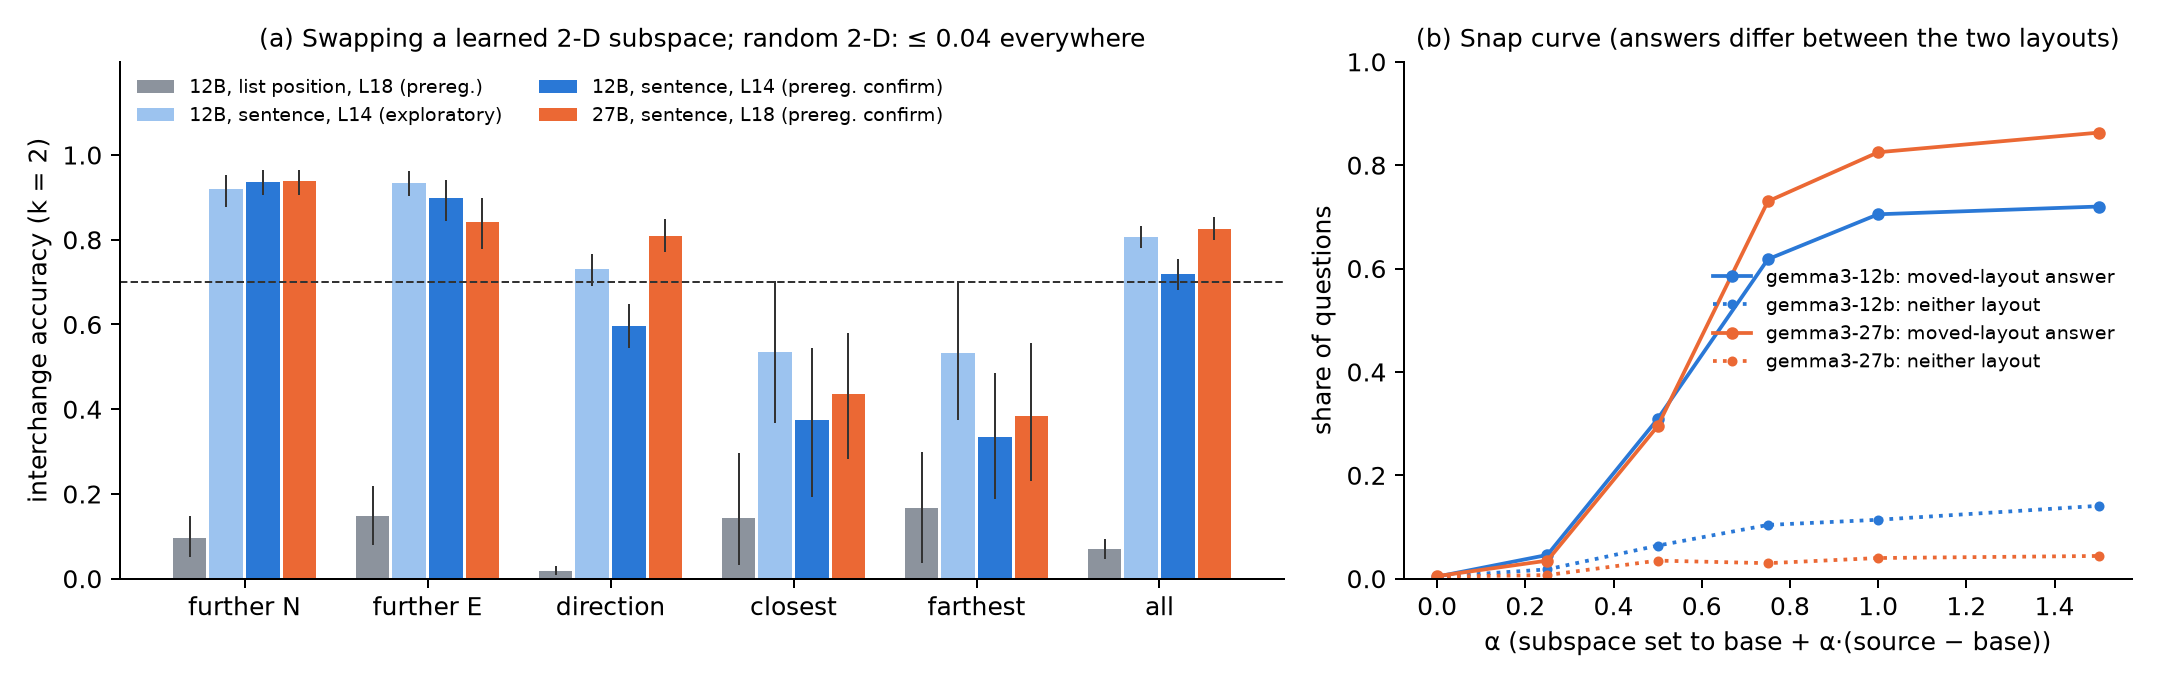
\includegraphics[width=1\linewidth,height=\textheight,keepaspectratio,alt={(a) Share of affected answers moved by a learned 2-D subspace, by question type. Grey: the object list. Blue and orange: the moved object's sentence, exploratory and preregistered runs. (b) As the subspace is set from the original value (α = 0) to the moved value (α = 1), answers switch abruptly from one stated layout to the other.}]{figures/fig4_code.png}
\caption{(a) Share of affected answers moved by a learned 2-D subspace,
by question type. Grey: the object list. Blue and orange: the moved
object's sentence, exploratory and preregistered runs. (b) As the
subspace is set from the original value (α = 0) to the moved value (α =
1), answers switch abruptly from one stated layout to the other.}
\end{figure}

\subsection{3.4 Why the map is not used}\label{why-the-map-is-not-used}

We now ask what the question reads, using chains R → M → C, where C is
placed relative to M and M relative to the root R.

\textbf{The question reads each object's own sentence, never the list.}
We blocked the question tokens from attending to one part of the prompt.
Blocking the object list, where the map lives, changes accuracy by at
most 0.018. Blocking C's own sentence costs questions about C and M
\textbf{0.35}, and blocking M's sentence costs questions about M and R
\textbf{0.41}. Nearly all of these effects come from layers 16--31.

\textbf{But it does not re-read the chain.} Questions about C and R need
M's offset. Yet blocking M's sentence costs them only \textbf{0.027
{[}0.017, 0.039{]}}. This rejects our preregistered hypothesis that the
question re-reads every sentence in the chain.

\textbf{The answers use the chain only partly.} If M's offset reaches
the question, it must come through C's sentence. So we copied C's
sentence, at every layer, from a scene where M (and therefore C) had
moved. This moved only \textbf{0.13 {[}0.09, 0.17{]}} of the answers. An
exploratory comparison shows why. We built pairs in which C ends up at
the same new position in two ways: either C's own sentence changes, or
only M's sentence changes. The geometry is identical, so a model that
fully combines the chain should update its answers equally often. It
does not. On questions about C and R, the model updates correctly in
\textbf{0.39} of cases when C's own sentence changes, but in only
\textbf{0.21} when only M's sentence changes. In most of the second kind
of case (72\%), it does not change its answer at all. The answers lean
on each object's own sentence and give the parent's offset about half
its weight.

\subsection{3.5 The map would have answered
better}\label{the-map-would-have-answered-better}

The map combines the chain correctly (§3.1), while the answers do not.
So answering from the map should beat the model, but only on questions
that need the chain. We decoded every object's position with the
layer-21 probe, answered each question geometrically from the decoded
positions, and compared these answers with the model's own on 300 new
chains (5,350 questions).

The map wins exactly where expected (Fig. 5). On questions about C and R
it scores \textbf{0.80 vs 0.73 for the model (difference +0.069
{[}+0.042, +0.094{]})}. On questions that need no chaining, the two tie
(0.91 vs 0.89 and 0.90 vs 0.90). Layer 24 shows the same pattern
(+0.056). The advantage depends on how well the probe reads the map: it
shrinks at layer 28 (+0.010) and reverses at layer 18, where the probe
is weakest.

\begin{figure}
\centering
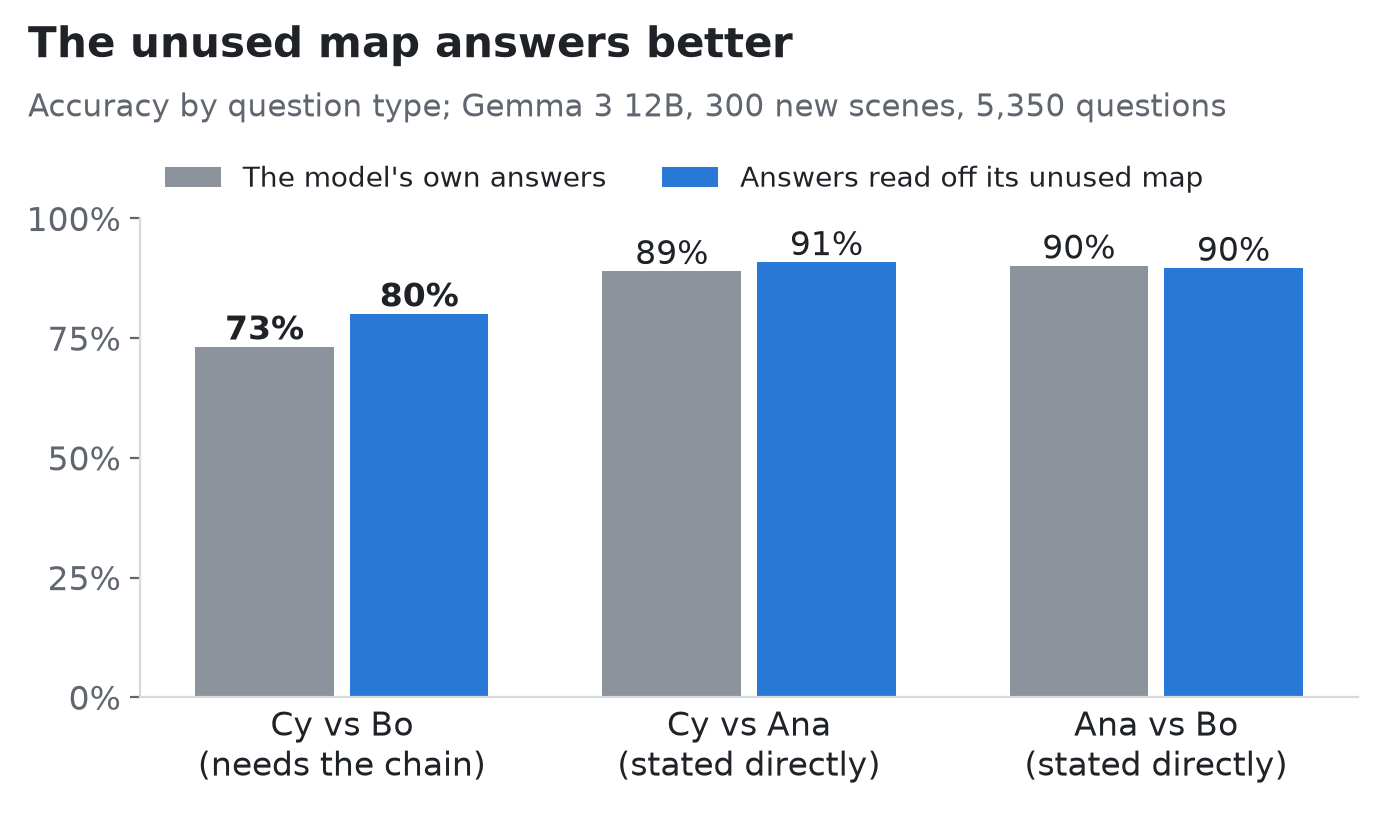
\includegraphics[width=1\linewidth,height=\textheight,keepaspectratio,alt={Accuracy of the model's own answers and of answers read off its unused map (layer 21), by question type.}]{figures/fig5_map_vs_model.png}
\caption{Accuracy of the model's own answers and of answers read off its
unused map (layer 21), by question type.}
\end{figure}

\textbf{Pointing attention at the map does not help.} If the map were
usable as it is, pushing the question to attend to it should improve
chain answers. We added a bias of +1 to +8 to the attention from the
question to the object names in the list (layers 16--31). A control
applied the same bias to the token just before each name. No bias
improved chain questions beyond the control. Strong biases hurt every
question type. The one effect specific to the map was harmful: it
lowered accuracy on questions about C and M by 0.049 (b = 2) and 0.136
(b = 4) beyond the control. Attending to the map distracts the question
from the sentence it normally reads, without giving it a better answer.

\section{4. Discussion}\label{discussion}

\textbf{Summary.} Gemma 3 builds an accurate map of the scene, combining
sentences and even computing distances. Its answers take a different
route. Each sentence is condensed into a compact, switch-like code, and
the question reads the codes of the objects it names in layers 16--31.
This route uses the chain of relations only partly. The map, built at
the object list, sits off that route. It can be erased without cost, and
it would answer chain questions more accurately than the model does.
This is a spatial instance of a gap reported for other kinds of world
state: a faithful internal state paired with an unfaithful read-out
(Feng, Russell \& Steinhardt, 2024).

\textbf{Decodability is not use.} Our probes pass every control we know
of, including a nonlinear target, yet they sit off the causal path.
Claims about ``world models'' in language models need an intervention on
the decoded representation, and ideally an erasure with a random control
(cf.~Hewitt \& Liang, 2019; Vafa et al., 2024). The contrast with
Tehenan et al.~(2025) fits this view. They steer answers along
\emph{relation} directions, and relation codes do steer answers in our
model too; coordinate codes do not. The same point runs through the old
debate on mental imagery, which was about whether depictive images do
work in reasoning, not whether they exist (Kosslyn et al., 1978;
Pylyshyn, 2002).

\textbf{Why build a map at all?} Our tests rule out one explanation: the
map is not a backup that the model falls back on, at least not in its
linear form. Erasing it everywhere costs nothing, even when chains are
long. Two explanations remain. The map may be a by-product of how the
model processes text in general. Or it may serve uses we did not test,
such as describing a scene. Our question types can all be answered by
chaining; questions that are hard to answer without a layout, such as
collinearity or containment, would test the second explanation. Since
attention alone cannot connect the map to the answers, a natural next
step is to ask whether light fine-tuning can.

\section{5. Limitations}\label{limitations}

\begin{itemize}
\tightlist
\item
  \textbf{Scope.} Two models of one family, small scenes, five question
  types, fixed templates and integer grids. Other model families failed
  the behaviour test.
\item
  \textbf{Linear erasure.} We removed only the linear subspace the list
  probe reads. Nonlinear or differently placed information may survive,
  so ``not used'' means not used in that subspace. The erasure,
  attention and map-answer tests were run on 12B only.
\item
  \textbf{Probe-based answers.} The map's answers come from a probe we
  trained on the true positions. They show that the information is
  present and easy to read, not that the model could use it without
  extra computation. The advantage also depends on the layer.
\item
  \textbf{Subspace methods.} The write-in recovers only 37\% of the copy
  edit, so a linear reading of the stated offset captures only part of
  the code.
\item
  \textbf{Exploratory analyses.} The distance probe, the 0.39 vs 0.21
  comparison and the stability, failure and competence analyses were not
  preregistered.
\item
  \textbf{Small classes.} Closest and farthest questions have wide
  intervals.
\end{itemize}

\section{6. Preregistration}\label{preregistration}

All rules are in \texttt{docs/preregistration*.md}, committed before the
corresponding data.

{\def\LTcaptype{none} % do not increment counter
\begin{longtable}[]{@{}
  >{\raggedright\arraybackslash}p{(\linewidth - 6\tabcolsep) * \real{0.2500}}
  >{\raggedright\arraybackslash}p{(\linewidth - 6\tabcolsep) * \real{0.2500}}
  >{\raggedright\arraybackslash}p{(\linewidth - 6\tabcolsep) * \real{0.2500}}
  >{\raggedright\arraybackslash}p{(\linewidth - 6\tabcolsep) * \real{0.2500}}@{}}
\toprule\noalign{}
\begin{minipage}[b]{\linewidth}\raggedright
Test
\end{minipage} & \begin{minipage}[b]{\linewidth}\raggedright
Prediction
\end{minipage} & \begin{minipage}[b]{\linewidth}\raggedright
Result
\end{minipage} & \begin{minipage}[b]{\linewidth}\raggedright
Verdict
\end{minipage} \\
\midrule\noalign{}
\endhead
\bottomrule\noalign{}
\endlastfoot
Behaviour gate & a model solves the task without reasoning & Gemma 3 12B
on 3 objects & met \\
Probes (P2) & coordinates readable, controls fail & R² 0.74 & met \\
Patching at the list (P3) & copying the map moves answers & 0.00 &
failed \\
Probe steering (P4) & answers follow the probe directions & 2\% of
sweeps & failed \\
DAS at the list (P4) & 2-D subspace controls answers (≥ 0.7) & 0.07 &
failed \\
DAS at the sentence (P4c) & ≥ 0.70, random ≤ 0.05 (12B, 27B) & 0.72,
0.83 & confirmed \\
Halfway test & in-between answers below chance → switch & 0.085, 0.055
vs 0.141 & switch \\
Chain transfer, one layer (E3) & C's sentence carries its position & ≤
0.07 & not carried \\
Natural encoding (P5a) & code is linear in the offset & R² 0.31 vs null
0.35 & no linear encoding \\
Write-in (P5b) & ≥ 50\% of the copy edit & 37\% & partial \\
Erasure, 3 objects (P5c) & erasing hurts beyond random & ≤ 0 & not
used \\
Erasure, 4--5 objects (P6) & erasing hurts deep questions & ≤ 0.023 &
still not used \\
Attention knockout (P7) & question re-reads the chain & 0.027 &
rejected; list not read \\
Multi-layer transfer (P8) & C's sentence carries its position & 0.13 &
partial \\
Map answers (P9) & map beats model on chain questions & 0.80 vs 0.73 &
map better \\
Attention boost (P10) & attending to the map helps & no gain & no
benefit \\
\end{longtable}
}

\textbf{Deviations.} A code review changed which model the unchanged
selection rule picked, from Gemma 3 27B to 12B. One chain experiment
(E2) also used a stricter question set defined after the data. In the
attention-knockout test, a classification bug dropped direction
questions about C and M before scoring. The verdicts rest on the other
classes, which were unaffected. Each deviation is dated in
\texttt{results/RESULTS.md}.

\section{AI assistance}\label{ai-assistance}

The author used Claude (Anthropic) to help write the experiment code,
run analyses, and draft and edit this text. The research questions, the
preregistered designs and decision rules, and the conclusions were set
and checked by the author, who takes responsibility for all content.
Every number comes from the result files in the public repository.

\section{Code and data}\label{code-and-data}

Code, preregistrations (with their commit history), and all result files
are available at https://github.com/ccgomezn/geometry-llm.

\section{References}\label{references}

\begin{itemize}
\tightlist
\item
  An, J., Yang, L., Wang, M., Lu, L., An, W., \& Yang, E. (2026). From
  Human Cognition to Neural Activations: Probing the Computational
  Primitives of Spatial Reasoning in LLMs. arXiv:2603.26323.
\item
  Engels, J., Michaud, E. J., Liao, I., Gurnee, W., \& Tegmark, M.
  (2024). Not All Language Model Features Are One-Dimensionally Linear.
  \emph{ICLR 2025}. arXiv:2405.14860.
\item
  Feng, J., Russell, S., \& Steinhardt, J. (2024). Monitoring Latent
  World States in Language Models with Propositional Probes.
  arXiv:2406.19501.
\item
  Geiger, A., Wu, Z., Potts, C., Icard, T., \& Goodman, N. (2024).
  Finding Alignments Between Interpretable Causal Variables and
  Distributed Neural Representations. \emph{CLeaR 2024}, PMLR 236,
  160--187. arXiv:2303.02536.
\item
  Gurnee, W., \& Tegmark, M. (2023). Language Models Represent Space and
  Time. \emph{ICLR 2024}. arXiv:2310.02207.
\item
  Hewitt, J., \& Liang, P. (2019). Designing and Interpreting Probes
  with Control Tasks. \emph{EMNLP-IJCNLP}, 2733--2743.
  doi:10.18653/v1/D19-1275
\item
  Kosslyn, S. M., Ball, T. M., \& Reiser, B. J. (1978). Visual images
  preserve metric spatial information: Evidence from studies of image
  scanning. \emph{JEP:HPP}, 4(1), 47--60. doi:10.1037/0096-1523.4.1.47
\item
  Makelov, A., Lange, G., Geiger, A., \& Nanda, N. (2024). Is This the
  Subspace You Are Looking for? An Interpretability Illusion for
  Subspace Activation Patching. \emph{ICLR 2024}. arXiv:2311.17030.
\item
  Pylyshyn, Z. W. (2002). Mental imagery: In search of a theory.
  \emph{BBS}, 25(2), 157--182. doi:10.1017/S0140525X02000043
\item
  Ravfogel, S., Elazar, Y., Gonen, H., Twiton, M., \& Goldberg, Y.
  (2020). Null It Out: Guarding Protected Attributes by Iterative
  Nullspace Projection. \emph{ACL 2020}, 7237--7256.
  doi:10.18653/v1/2020.acl-main.647. arXiv:2004.07667.
\item
  Tehenan, M., Bolivar Moya, C., Long, T., \& Lin, G. (2025). Linear
  Spatial World Models Emerge in Large Language Models.
  arXiv:2506.02996.
\item
  Vafa, K., Chen, J. Y., Rambachan, A., Kleinberg, J., \& Mullainathan,
  S. (2024). Evaluating the World Model Implicit in a Generative Model.
  \emph{NeurIPS 2024}. arXiv:2406.03689.
\end{itemize}

\end{document}
